%--------------------------------------
% Solução Proposta
%--------------------------------------
\section{Solução Proposta}
\label{sec:solucao-proposta}


\todo[inline]{\textbf{NOTA}: Deve-se apresentar a visão geral da solução proposta, nesta seção você deve apresentar metodologia do trabalho ou procedimentos metodológicos – deve constar o instrumental, os métodos e as técnicas aplicados para a elaboração do trabalho.}


%--------------------------------------
% Arquitetura
%--------------------------------------
\subsection{Arquitetura}

\todo[inline]{\textbf{NOTA}: Deve-se apresentar uma visão geral da solução proposta, exemplo, usando uma Big Picture. Abaixo segue um \textbf{exemplo}.} 

A Figura~\ref{fig_bigpicture} apresenta uma visão geral da solução proposta que visa o desenvolvimento e análise de uma sistema de irrigação usando tecnologias de IoT.

\begin{figure}[h!]    
	\begin{center}
	    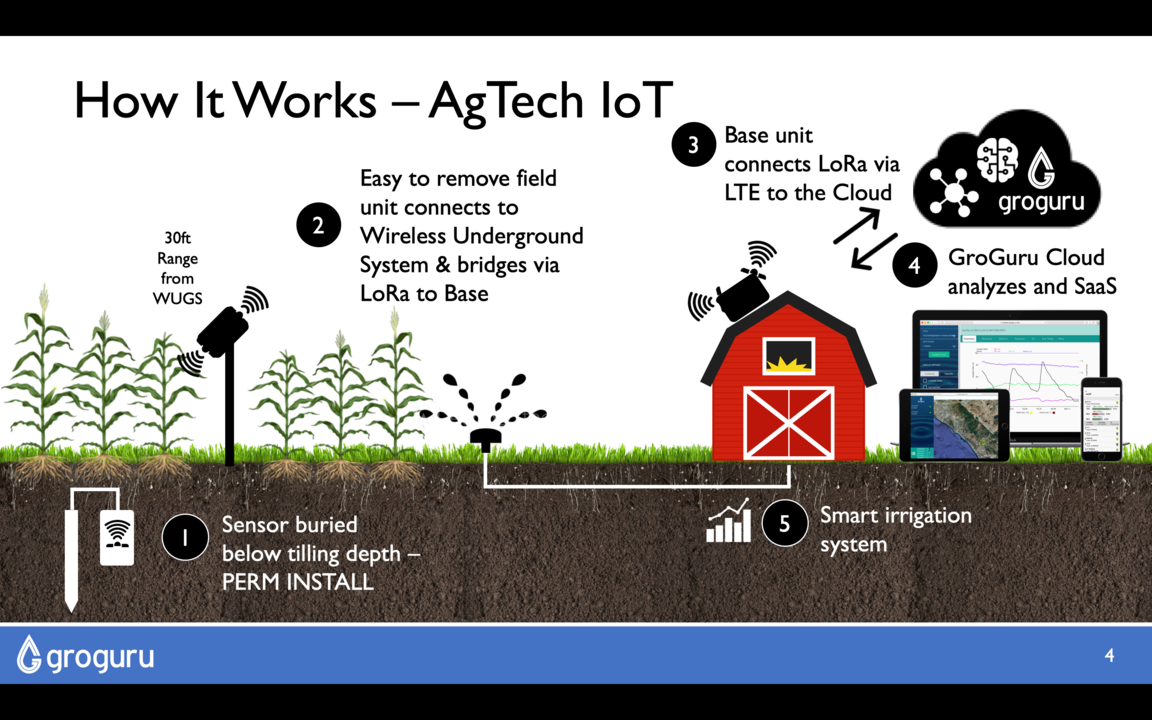
\includegraphics[scale=0.3]{imagens/bigpicture.png}
	\end{center}
	\caption{\label{fig_bigpicture}Como funciona o sistema de irrigação.}
\end{figure}

\todo[inline]{\textbf{NOTA}: Nesta seção, também deve-se apresentar o fluxo da sua solução, ou seja, um diagrama contendo os artefatos de entrada e saída para cada etapa da solução proposta. Um modelo de digrama que pode ser utilizado é o BPMN (http://www.bpmn.org). Abaixo segue um \textbf{exemplo}.}

A Figura~\ref{fig_digflow} apresenta o fluxo de execução da solução proposta contendo suas respectivas entradas e artefatos gerados no modelo BPMN.

\begin{figure}[h!]	
	\begin{center}
	    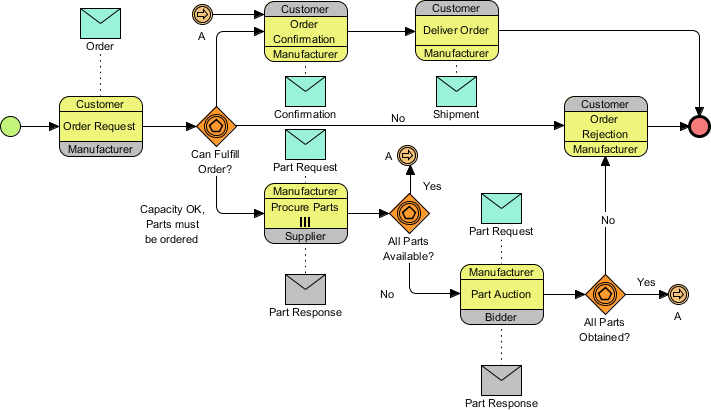
\includegraphics[scale=0.7]{imagens/34-final-business-process-diagram.png}
	\end{center}
    \caption{\label{fig_digflow}Diagram de fluxo no modelo BPMN.}
\end{figure}


%--------------------------------------
% Modelagem e Análise
%--------------------------------------
\subsection{Modelagem e Análise}
\label{sec:modelagem-analise}

\todo[inline]{Nesta subseção, apresenta-se um panorama da arquitetura da solução, destacando os principais componentes, entidades e interações. Deve-se adotar pelo menos um tipo de modelagem.}

\textcolor{red}{Exemplo: A solução proposta é composta por três módulos principais: (i) Interface do Usuário, (ii) Módulo de Processamento de Regras, e (iii) Gerenciador de Requisições. A comunicação entre os módulos é realizada por meio de eventos assíncronos. Para garantir a corretude das interações, utilizou-se modelagem formal com base em UML e Autômatos Finitos.}


\subsubsection{Modelagem com UML}

\textcolor{red}{Nesta parte, são apresentados os diagramas estruturais e comportamentais relevantes (e.g., casos de uso, atividades, estados, sequência, classes).}

\textcolor{red}{Exemplo:
%
A Figura 1 apresenta o Diagrama de Casos de Uso, onde é possível identificar os principais atores do sistema e suas interações com as funcionalidades.
A Figura 2 ilustra o Diagrama de Estados do componente Gerenciador de Requisições, evidenciando os estados "Inativo", "Aguardando Resposta" e "Erro de Timeout".}


\subsubsection{Modelagem com Autômatos Finitos}

\textcolor{red}{Aqui, são modelados formalmente os comportamentos dos módulos ou protocolos envolvidos, usando autômatos finitos determinísticos ou não determinísticos.}

\textcolor{red}{Exemplo:
%
O comportamento do módulo de autenticação foi modelado como um Autômato Finito Determinístico (AFD), conforme ilustrado na Figura 3.
O autômato possui os seguintes estados: q0 (esperando credenciais), q1 (verificação em andamento), q2 (acesso permitido), e q3 (acesso negado).
A transição de q0 para q1 ocorre ao receber um par usuário/senha; a transição para q2 ou q3 depende do resultado da verificação.}


\subsubsection{Modelagem com Redes de Petri}

\textcolor{red}{Utilize Redes de Petri para modelar e analisar aspectos concorrentes, sincronização e condições de deadlock.}

\textcolor{red}{Exemplo:
%
Para representar o processo de requisição e resposta entre cliente e servidor, modelamos o sistema utilizando uma Rede de Petri (Figura 4).
A rede inclui lugares como ClientePronto, RequisiçãoEnviada, ServidorOcupado e transições como EnviarRequisição, ProcessarRequisição, e ResponderCliente.
Foi verificada a ausência de deadlocks e a reentrância do sistema, assegurando que sempre será possível retornar ao estado inicial após uma interação completa.}


\subsubsection{Análise de Corretude}

\todo[inline]{\textbf{NOTA}: Aqui, discute-se os limites da modelagem, possíveis extensões e como os resultados reforçam a confiança na solução.}

\textcolor{red}{Apresente aqui os critérios de análise formal e os resultados obtidos com base nos modelos apresentados. Você pode usar ferramentas de verificação (ex: SPIN, TINA, NuSMV, UPPAAL) ou provas matemáticas.
%
Exemplo: A partir do modelo em autômatos, foi possível aplicar a verificação de propriedades de segurança e vivacidade.
Utilizando a ferramenta NuSMV, especificamos as propriedades desejadas em LTL (Linear Temporal Logic), como: $G(request -> F(response))$ - toda requisição será eventualmente respondida; $G \neg deadlock$ - ausência de deadlock em qualquer execução do sistema.
Todas as propriedades foram satisfatóriamente verificadas, confirmando a corretude formal da solução.}

\textcolor{red}{A modelagem revelou potenciais condições de corrida entre os módulos de log e autenticação, levando à introdução de um mecanismo adicional de controle de concorrência.
A utilização de três diferentes abordagens formais (UML, Autômatos, e Redes de Petri) permitiu uma análise multifacetada do sistema, contemplando tanto aspectos estruturais quanto comportamentais.}


\subsection{Ambiente de Desenvolvimento e Implementação da Solução}

\todo[inline]{\textbf{NOTA}: Deve-se apresentar as ferramentas já pesquisadas que serão adotadas na solução propostas, bem como, explicar como as ferramentas serão correlacionadas. \textbf{Importante}, mencionar o nome da ferramenta, versão e onde pode ser encontrada, segue um pequeno \textbf{exemplo} de uso.}

\textcolor{red}{Exemplo: A solução proposta será uma ferramenta de verificação de código implementada como um transformador de código escrita em C/C++ usando o \textit{framework} para compiladores LLVM~\footnote{https://llvm.org/} (v$6.0$). A solução utilizará como \textit{front-end} para programas escritos em C o Clang~\footnote{https://clang.llvm.org/} (v$6.0$ para gerar código LLVM-bitcode que será usado para a transformação de código. As ferramentas LibFuzzer (v$6.0$) e KLEE (v$2.0$) serão utilizadas para gerar entrada de testes para os códigos que serão analisados. Finalmente, o MetaSMT (v$4.rc2$) será usado como API para motores de solucionadores de satisfabilidade.}



